\documentclass[aspectratio=169,11pt]{beamer}

% =========================================================
% Packages
% =========================================================
\usepackage{amsmath,amssymb,mathtools,bm}
\usepackage{booktabs}
\usepackage{array}
\usepackage{ragged2e}
\usepackage{microtype}
\usepackage{graphicx}
\usepackage{xcolor}
\usepackage{tikz}
\usetikzlibrary{arrows.meta,positioning}
\usepackage{pgfplots}
\pgfplotsset{compat=1.18}

% =========================================================
% Theme
% =========================================================
\usetheme{Boadilla}
\usecolortheme{default}
\setbeamertemplate{navigation symbols}{}
\setbeamertemplate{footline}[frame number]

\definecolor{DeepBlue}{RGB}{28,66,120}
\definecolor{DarkGray}{RGB}{55,55,55}
\definecolor{SoftGray}{RGB}{242,242,242}
\definecolor{DarkRed}{RGB}{155,45,45}
\definecolor{DarkGreen}{RGB}{35,110,75}

\setbeamercolor{structure}{fg=DeepBlue}
\setbeamercolor{frametitle}{fg=DeepBlue}
\setbeamercolor{title}{fg=DeepBlue}
\setbeamercolor{block title}{bg=DeepBlue!12,fg=DeepBlue}
\setbeamercolor{block body}{bg=DeepBlue!3,fg=black}
\setbeamercolor{alerted text}{fg=DarkRed}

% =========================================================
% Layout tuning (compact vertical rhythm)
% =========================================================
\setbeamersize{text margin left=1.1em,text margin right=1.1em}

\AtBeginDocument{%
  \setlength{\abovedisplayskip}{3.5pt plus 2pt minus 1.5pt}%
  \setlength{\belowdisplayskip}{3.5pt plus 2pt minus 1.5pt}%
  \setlength{\abovedisplayshortskip}{1.5pt plus 1pt minus 1pt}%
  \setlength{\belowdisplayshortskip}{2.5pt plus 1pt minus 1pt}%
  \setlength{\jot}{2pt}%
}

\addtobeamertemplate{block begin}{\vspace{-0.45em}}{}
\addtobeamertemplate{block end}{}{\vspace{-0.35em}}
\addtobeamertemplate{block alerted begin}{\vspace{-0.45em}}{}
\addtobeamertemplate{block alerted end}{}{\vspace{-0.35em}}

\setlength{\leftmargini}{1.5em}
\setbeamertemplate{itemize/enumerate body begin}{\vspace{-0.2em}}
\setbeamertemplate{itemize/enumerate body end}{\vspace{-0.2em}}

\setbeamerfont{frametitle}{size=\large,series=\bfseries}

\newcommand{\NoHyph}{\hyphenpenalty=10000\exhyphenpenalty=10000\relax}
\newcolumntype{L}[1]{>{\RaggedRight\NoHyph\arraybackslash}p{#1}}
\newcolumntype{B}[1]{>{\RaggedRight\NoHyph\bfseries\arraybackslash}p{#1}}

% =========================================================
% Commands
% =========================================================
\newcommand{\E}{\mathbb{E}}
\newcommand{\Var}{\operatorname{Var}}
\newcommand{\Cov}{\operatorname{Cov}}
\DeclareMathOperator*{\argmin}{arg\,min}
\DeclareMathOperator*{\plim}{plim}
\newcommand{\pto}{\xrightarrow{\;p\;}}
\newcommand{\dto}{\xrightarrow{\;d\;}}
\newcommand{\PrfLbl}{\textcolor{DeepBlue}{\textit{Proof.}}\ }
\newcommand{\QED}{\hfill$\square$}
\newcommand{\Src}[1]{{\scriptsize\textcolor{DarkGray}{#1}}}
% Section sign from the math font: the text-mode \S uses a TS1 sans font
% that is only available as a bitmap without cm-super, which breaks
% microtype's font expansion on some local TeX installations.
\newcommand{\Sec}{\ensuremath{\S}}

% =========================================================
% Title
% =========================================================
\title{Mostly Harmless Econometrics}
\subtitle{
\textbf{Chapter 3.1: Regression Fundamentals}
\\[0.55em]
The CEF
$\rightarrow$ Population regression
$\rightarrow$ Why regression?
$\rightarrow$ Asymptotic inference
}
\author{Kaiwen Luo}
\institute{Washington University in St.Louis}
\date{\today}

\begin{document}

% =========================================================
\begin{frame}
    \titlepage
\end{frame}


% ------------------------------------------------------------
\begin{frame}{Where We Are}
\small

\begin{itemize}
    \item \textbf{Chapter 2:} regression as a \emph{computational device} for
    estimating treatment--control differences in an experiment, with and
    without covariates. In the class-size study (\Sec{}2.3) the regressor was
    randomly assigned $\Rightarrow$ the estimates are causal.
    \item \textbf{Most studies:} regression is run on \alert{observational data}.
    Without random assignment, estimates may or may not be causal
    ($\rightarrow$ \Sec{}3.2).
    \item \textbf{This section:} set causality aside and study the
    \emph{mechanical} properties of regression --- universal features of the
    population regression vector and its sample analog that have nothing to
    do with how the researcher interprets the output.
\end{itemize}

\medskip

\begin{center}
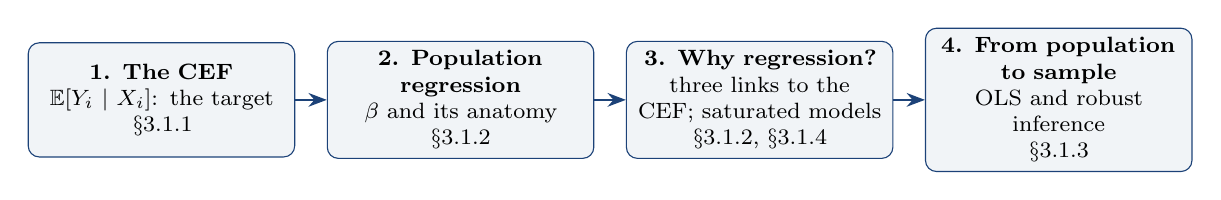
\begin{tikzpicture}[
    node distance=4mm,
    box/.style={draw=DeepBlue, fill=DeepBlue!6, rounded corners,
                align=center, text width=3.15cm, minimum height=1.45cm,
                font=\footnotesize, execute at begin node=\NoHyph},
    arr/.style={-{Stealth}, thick, DeepBlue}]
  \node[box] (cef) {\textbf{1. The CEF}\\ $\E[Y_i\mid X_i]$: the target\\ \Sec{}3.1.1};
  \node[box, right=of cef] (reg) {\textbf{2. Population regression}\\ $\beta$ and its anatomy\\ \Sec{}3.1.2};
  \node[box, right=of reg] (why) {\textbf{3. Why regression?}\\ three links to the CEF; saturated models\\ \Sec{}3.1.2, \Sec{}3.1.4};
  \node[box, right=of why] (inf) {\textbf{4. From population to sample}\\ OLS and robust inference\\ \Sec{}3.1.3};
  \draw[arr] (cef) -- (reg);
  \draw[arr] (reg) -- (why);
  \draw[arr] (why) -- (inf);
\end{tikzpicture}
\end{center}

\end{frame}


% ============================================================
% SECTION 1: THE CEF
% ============================================================

\section{The Conditional Expectation Function}

% ------------------------------------------------------------
\begin{frame}{Motivation: ``Systematic Randomness''}
\small

\begin{itemize}
    \item Empirical labor economics studies differences between people that
    might account for differences in their economic fortunes.
    \item These differences are notoriously hard to explain --- in a word,
    \emph{random}. But randomness can be summarized and interpreted in a
    useful way.
    \item \textbf{Example:} schooling and earnings. On average, people with
    more schooling earn more. The connection has considerable predictive
    power despite enormous variation in individual circumstances.
\end{itemize}

\begin{alertblock}{Prediction $\neq$ causation}
That more educated people earn more does not mean that schooling
\emph{causes} earnings to increase. The causal question is of enormous
importance and recurs throughout the book --- but even without resolving it,
education predicts earnings in a narrow statistical sense.
\end{alertblock}

\medskip

\[
\boxed{
\text{This predictive power is compellingly summarized by the
\textbf{conditional expectation function} (CEF).}
}
\]

\end{frame}


% ------------------------------------------------------------
\begin{frame}{The Conditional Expectation Function}
\small

\begin{block}{Definition}
For a dependent variable $Y_i$ and a $K\times1$ covariate vector $X_i$
(elements $x_{ki}$), the CEF $\E[Y_i\mid X_i]$ is the expectation, or
population average, of $Y_i$ with $X_i$ held fixed --- the mean in an
infinitely large sample, or the average in a completely enumerated finite
population. At a specific value $X_i=x$:
\[
\underbrace{\E[Y_i\mid X_i=x] = \int t\, f_y(t\mid X_i=x)\,dt}_{Y_i \text{ continuous, conditional density } f_y}
\qquad\qquad
\underbrace{\E[Y_i\mid X_i=x] = \sum_t t\, P(Y_i=t\mid X_i=x)}_{Y_i \text{ discrete, conditional pmf}}
\]
\end{block}

\begin{itemize}
    \item $\E[Y_i\mid X_i]$ is a \emph{function of $X_i$}; since $X_i$ is
    random, the CEF is random. Sometimes we use one value, e.g.\
    $\E[Y_i\mid X_i=42]$.
    \item Chapter 2 special case: $\E[Y_i\mid D_i]$, $D_i\in\{0,1\}$, takes
    two values; usually we want CEFs of many variables, collected in $X_i$.
\end{itemize}

\begin{block}{``Population first''}
Expectation is a population concept; samples are used to learn about it
(\Sec{}3.1.3). \alert{Define the objects of interest before
using data to study them.} \Src{(Chamberlain 1984; Goldberger 1991; Manski 1991)}
\end{block}

\end{frame}


% ------------------------------------------------------------
\begin{frame}{Example: The CEF of Log Wages Given Schooling (Fig.\ 3.1.1)}
\small

\begin{columns}[T]
\begin{column}{0.57\textwidth}
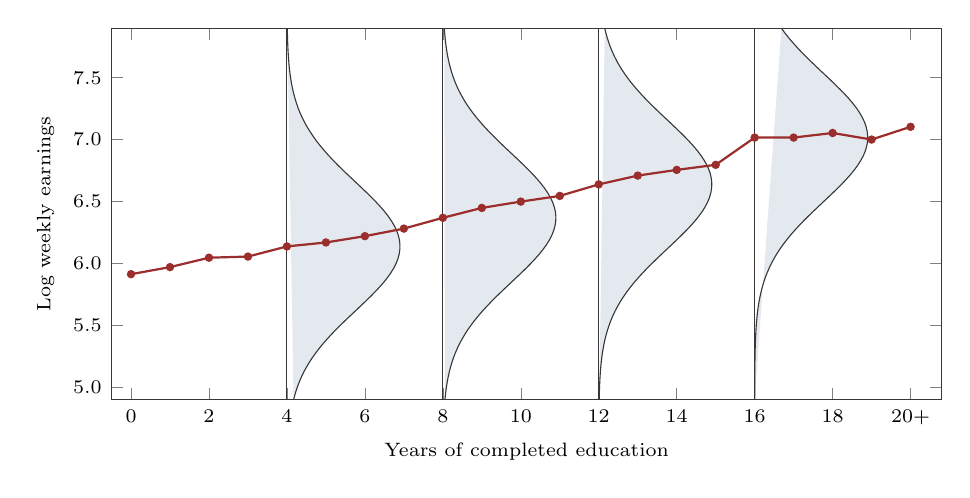
\begin{tikzpicture}
\begin{axis}[
    width=\linewidth, height=6.3cm,
    xmin=-0.5, xmax=20.8, ymin=4.9, ymax=7.9,
    xtick={0,2,...,20},
    xticklabels={0,2,4,6,8,10,12,14,16,18,20+},
    ytick={5.0,5.5,6.0,6.5,7.0,7.5},
    yticklabel style={/pgf/number format/.cd,fixed,fixed zerofill,precision=1},
    tick label style={font=\scriptsize},
    label style={font=\scriptsize},
    xlabel={Years of completed education},
    ylabel={Log weekly earnings},
    axis line style={DarkGray},
]
  % stylized conditional distributions at s = 4, 8, 12, 16
  \addplot[draw=DarkGray, fill=DeepBlue!12, domain=4.9:7.9, samples=80, variable=\t]
      ({4+2.9*exp(-((\t-6.138)^2)/(2*0.52^2))}, {\t});
  \addplot[draw=DarkGray, fill=DeepBlue!12, domain=4.9:7.9, samples=80, variable=\t]
      ({8+2.9*exp(-((\t-6.369)^2)/(2*0.52^2))}, {\t});
  \addplot[draw=DarkGray, fill=DeepBlue!12, domain=4.9:7.9, samples=80, variable=\t]
      ({12+2.9*exp(-((\t-6.639)^2)/(2*0.52^2))}, {\t});
  \addplot[draw=DarkGray, fill=DeepBlue!12, domain=4.9:7.9, samples=80, variable=\t]
      ({16+2.9*exp(-((\t-7.017)^2)/(2*0.52^2))}, {\t});
  \draw[DarkGray] (axis cs:4,4.9) -- (axis cs:4,7.9);
  \draw[DarkGray] (axis cs:8,4.9) -- (axis cs:8,7.9);
  \draw[DarkGray] (axis cs:12,4.9) -- (axis cs:12,7.9);
  \draw[DarkGray] (axis cs:16,4.9) -- (axis cs:16,7.9);
  % CEF
  \addplot[DarkRed, thick, mark=*, mark size=1.1pt] coordinates {
      (0,5.914) (1,5.971) (2,6.047) (3,6.056) (4,6.138) (5,6.170)
      (6,6.221) (7,6.282) (8,6.369) (9,6.449) (10,6.500) (11,6.546)
      (12,6.639) (13,6.710) (14,6.756) (15,6.797) (16,7.017) (17,7.017)
      (18,7.054) (19,7.001) (20,7.104)};
\end{axis}
\end{tikzpicture}

\vspace{-0.3em}
\Src{Schematic: CEF values approximated from MHE Fig.\ 3.1.2;
conditional distributions are stylized.}
\end{column}

\begin{column}{0.41\textwidth}
\begin{block}{Data}
White men aged 40--49, 1980 Census (IPUMS 5\% file). Red line: average log
weekly wages at each schooling level. Shaded: the distribution of earnings at
4, 8, 12, and 16 years of schooling.
\end{block}

\medskip

\begin{block}{What the CEF shows}
\begin{itemize}
    \item Enormous variation in earnings \emph{within} each schooling level.
    \item Even so, people with more schooling generally earn more.
    \item The average earnings gain per year of schooling is typically
    about \alert{10 percent}.
\end{itemize}
\end{block}
\end{column}
\end{columns}

\end{frame}


% ------------------------------------------------------------
\begin{frame}{The Law of Iterated Expectations}
\small

An unconditional expectation is the unconditional average of the CEF:
\[
\boxed{\E[Y_i] = \E\{\E[Y_i\mid X_i]\}}
\tag{3.1.1}
\]
where the outer expectation uses the distribution of $X_i$.

\PrfLbl (continuous case). Let $f_{xy}(u,t)$ be the joint density of
$(X_i,Y_i)$, $f_y(t\mid X_i=u)$ the conditional density of $Y_i$ given
$X_i=u$, and $g_x(u)$, $g_y(t)$ the marginal densities. Then
\[
\begin{aligned}
\E\{\E[Y_i\mid X_i]\}
&= \int \E[Y_i\mid X_i=u]\,g_x(u)\,du
 = \int\Big[\int t\,f_y(t\mid X_i=u)\,dt\Big]g_x(u)\,du \\
&= \int\!\!\int t\,f_y(t\mid X_i=u)\,g_x(u)\,du\,dt
 = \int t\Big[\int f_y(t\mid X_i=u)\,g_x(u)\,du\Big]dt \\
&= \int t\Big[\int f_{xy}(u,t)\,du\Big]dt
 = \int t\,g_y(t)\,dt = \E[Y_i]. \qquad\square
\end{aligned}
\]

\begin{block}{Intuition}
Average earnings among men and women $=$ (average for men)$\times$(share male)
$+$ (average for women)$\times$(share female).
\end{block}

\medskip
Its power: it breaks a random variable into two pieces --- the CEF and a
residual with special properties.

\end{frame}


% ------------------------------------------------------------
\begin{frame}{Property 1: Decomposition}
\small

\begin{block}{Theorem 3.1.1 (The CEF Decomposition Property)}
\[
Y_i = \E[Y_i\mid X_i] + \varepsilon_i,
\]
where (i) $\varepsilon_i$ is mean independent of $X_i$, that is,
$\E[\varepsilon_i\mid X_i]=0$; and therefore (ii) $\varepsilon_i$ is
uncorrelated with any function of $X_i$.
\end{block}

\medskip

\PrfLbl
\begin{enumerate}
    \item[(i)] $\E[\varepsilon_i\mid X_i]
    = \E\big[Y_i-\E[Y_i\mid X_i]\,\big|\,X_i\big]
    = \E[Y_i\mid X_i]-\E[Y_i\mid X_i] = 0.$
    \item[(ii)] Let $h(X_i)$ be any function of $X_i$. By iterated
    expectations,
    $\E[h(X_i)\varepsilon_i] = \E\{h(X_i)\,\E[\varepsilon_i\mid X_i]\}$,
    which is $0$ by mean independence. \QED
\end{enumerate}

\medskip

\begin{block}{Interpretation}
Any random variable $Y_i$ splits into
\begin{itemize}
    \item a piece ``explained by $X_i$'' --- the CEF; and
    \item a leftover piece that is orthogonal to (uncorrelated with)
    \emph{any} function of $X_i$.
\end{itemize}
\end{block}

\end{frame}


% ------------------------------------------------------------
\begin{frame}{Property 2: Prediction}
\small

Why is the CEF a good summary of how $Y_i$ relates to $X_i$? Averages are
natural representative values --- and, formally, the CEF solves a
\emph{minimum mean squared error} (MMSE) prediction problem.

\begin{block}{Theorem 3.1.2 (The CEF Prediction Property)}
Let $m(X_i)$ be any function of $X_i$. The CEF solves
\[
\E[Y_i\mid X_i] = \argmin_{m(X_i)} \E\big[(Y_i-m(X_i))^2\big],
\]
so it is the MMSE predictor of $Y_i$ given $X_i$.
\end{block}

\PrfLbl
\[
\begin{aligned}
(Y_i-m(X_i))^2
&= \big((Y_i-\E[Y_i\mid X_i]) + (\E[Y_i\mid X_i]-m(X_i))\big)^2 \\
&= \underbrace{(Y_i-\E[Y_i\mid X_i])^2}_{\text{no } m(\cdot)}
 + \underbrace{2(\E[Y_i\mid X_i]-m(X_i))\,(Y_i-\E[Y_i\mid X_i])}_{h(X_i)\varepsilon_i}
 + \underbrace{(\E[Y_i\mid X_i]-m(X_i))^2}_{\geq 0}.
\end{aligned}
\]
The middle term has expectation zero by the decomposition property, with
$h(X_i)\equiv 2(\E[Y_i\mid X_i]-m(X_i))$; the last term is minimized (at zero)
when $m(X_i)$ is the CEF. \QED

\end{frame}


% ------------------------------------------------------------
\begin{frame}{Property 3: Analysis of Variance}
\small

\begin{block}{Theorem 3.1.3 (The ANOVA Theorem)}
\[
\Var(Y_i) = \Var\big(\E[Y_i\mid X_i]\big) + \E\big[\Var(Y_i\mid X_i)\big],
\]
where $\Var(Y_i\mid X_i)$ is the conditional variance of $Y_i$ given $X_i$.
\end{block}

\PrfLbl By the decomposition property, $\varepsilon_i\equiv Y_i-\E[Y_i\mid X_i]$
and $\E[Y_i\mid X_i]$ are uncorrelated, so $\Var(Y_i)$ is the variance of the
CEF plus the variance of $\varepsilon_i$. The latter is
\[
\E[\varepsilon_i^2] = \E\big[\E[\varepsilon_i^2\mid X_i]\big]
= \E\big[\Var(Y_i\mid X_i)\big],
\]
since $\E[\varepsilon_i^2\mid X_i]=\Var(Y_i\mid X_i)$ when
$\varepsilon_i\equiv Y_i-\E[Y_i\mid X_i]$. \QED

\medskip

\begin{itemize}
    \item Familiar from the ANOVA table in regression output.
    \item Inequality research: decompose changes in the income distribution
    into changes in worker characteristics and changes in what is left over
    \Src{(e.g., Autor, Katz, and Kearney 2005)}.
\end{itemize}

\begin{alertblock}{Perhaps less familiar}
The two CEF properties and the ANOVA decomposition hold in the population as
well as in samples, and do \alert{not} require a linear CEF. In fact, the
validity of linear regression as an empirical tool does not turn on
linearity either.
\end{alertblock}

\end{frame}


% ============================================================
% SECTION 2: POPULATION REGRESSION
% ============================================================

\section{Population Regression}

% ------------------------------------------------------------
\begin{frame}{The Population Regression Vector}
\small

``So what's the regression you want to run?'' Regression is a valuable
baseline for almost all empirical work because it is tightly linked to the
CEF. To make the link precise, first define the object --- with
\alert{no causal content yet}.

\begin{block}{Definition: population regression coefficients ($K\times1$)}
\[
\beta = \argmin_b \E\big[(Y_i-X_i'b)^2\big]
\tag{3.1.2}
\]
First-order condition:
$\E\big[X_i(Y_i-X_i'b)\big]=0
\;\Longrightarrow\;
\boxed{\beta = \E[X_iX_i']^{-1}\E[X_iY_i]}$
\end{block}

\begin{itemize}
    \item Population residual $e_i\equiv Y_i-X_i'\beta$. By construction
    $\E[X_ie_i]=\E[X_i(Y_i-X_i'\beta)]=0$: the residual is uncorrelated with
    the regressors.
    \item Bivariate case (one regressor $x_i$ plus a constant):
    \[
    \beta_1 = \frac{\Cov(Y_i,x_i)}{\Var(x_i)},
    \qquad
    \alpha = \E[Y_i]-\beta_1\E[x_i].
    \]
\end{itemize}

\begin{alertblock}{The residual has no life of its own}
$e_i$ owes its existence and meaning to $\beta$; it is not a structural
error term ($\rightarrow$ causal regression in \Sec{}3.2).
\end{alertblock}

\end{frame}


% ------------------------------------------------------------
\begin{frame}{Regression Anatomy}
\small

With more than one non-constant regressor, the slope on the $k$th regressor is
\[
\boxed{
\beta_k = \frac{\Cov(Y_i,\tilde x_{ki})}{\Var(\tilde x_{ki})}
}
\tag{3.1.3}
\]
where $\tilde x_{ki}$ is the residual from a regression of $x_{ki}$ on
\emph{all the other covariates}.

\medskip

\begin{itemize}
    \item $\E[X_iX_i']^{-1}\E[X_iY_i]$ is the $K\times1$ vector whose $k$th
    element is $\Cov(Y_i,\tilde x_{ki})/\Var(\tilde x_{ki})$.
    \item This ``anatomy'' reveals much more than the matrix formula:
    \alert{each coefficient in a multivariate regression is the bivariate
    slope for that regressor after partialing out all the other covariates.}
\end{itemize}

\medskip

\PrfLbl Substitute
$Y_i = \alpha + \beta_1x_{1i}+\cdots+\beta_kx_{ki}+\cdots+\beta_Kx_{Ki}+e_i$
into $\Cov(Y_i,\tilde x_{ki})$:
\begin{enumerate}
    \item $\tilde x_{ki}$ is a linear combination of the regressors
    $\Rightarrow$ uncorrelated with $e_i$;
    \item $\tilde x_{ki}$ is a residual from a regression on the other
    covariates $\Rightarrow$ uncorrelated with each of them;
    \item for the same reason, $\Cov(\tilde x_{ki},x_{ki})=\Var(\tilde x_{ki})$.
\end{enumerate}
Hence $\Cov(Y_i,\tilde x_{ki})=\beta_k\Var(\tilde x_{ki})$. \QED

\end{frame}


% ------------------------------------------------------------
\begin{frame}{Regression Anatomy: Remarks}
\small

\begin{itemize}
    \item Usually attributed to \textbf{Frisch and Waugh (1933)}.
    \item \textbf{Alternative version:}
    $\beta_k = \Cov(\tilde Y_{ki},\tilde x_{ki})/\Var(\tilde x_{ki})$, where
    $\tilde Y_{ki}$ is the residual from regressing $Y_i$ on every covariate
    except $x_{ki}$. It works because the fitted values removed from
    $\tilde Y_{ki}$ are uncorrelated with $\tilde x_{ki}$.
    \item \textbf{Visualization:} the least squares slope in a scatterplot of
    $\tilde Y_{ki}$ against $\tilde x_{ki}$ is the multivariate $\beta_k$,
    even though the plot is two-dimensional.
    \item \textbf{Pitfall:} partialing the other covariates out of $Y_i$
    \emph{only} is not enough:
    \[
    \frac{\Cov(\tilde Y_{ki},x_{ki})}{\Var(x_{ki})}
    = \left[\frac{\Cov(\tilde Y_{ki},\tilde x_{ki})}{\Var(\tilde x_{ki})}\right]
      \left[\frac{\Var(\tilde x_{ki})}{\Var(x_{ki})}\right]
    \neq \beta_k,
    \]
    unless $x_{ki}$ is uncorrelated with the other covariates.
\end{itemize}

\begin{block}{Population parameters, not estimators}
These coefficients are \emph{nonstochastic} features of the joint
distribution of $Y_i$ and $X_i$ --- what you would see with a complete
enumeration of the population (or knowledge of the data-generating process).
Think about what a parameter means \emph{before} worrying about estimation.
\end{block}

\end{frame}


% ============================================================
% SECTION 3: WHY REGRESSION?
% ============================================================

\section{Why Regression? Regression and the CEF}

% ------------------------------------------------------------
\begin{frame}{Three Reasons to Care About $\beta$}
\small

The link between the regression function --- the best-fitting line from
minimizing expected squared errors --- and the CEF can be explained in at
least three ways:

\medskip

\begin{center}
\renewcommand{\arraystretch}{1.35}
\begin{tabular}{@{}B{3.6cm}L{5.7cm}L{4.6cm}@{}}
\toprule
Justification & Statement & Scope \\
\midrule
I.\ Linear CEF \newline (Thm 3.1.4)
  & If $\E[Y_i\mid X_i]$ is linear, the population regression function
    \emph{is} the CEF.
  & Special cases: joint normality, saturated models. \\
II.\ Best linear predictor \newline (Thm 3.1.5)
  & $X_i'\beta$ is the MMSE \emph{linear} predictor of $Y_i$.
  & Always holds. \\
III.\ Regression CEF \newline (Thm 3.1.6)
  & $X_i'\beta$ is the MMSE linear \emph{approximation} to
    $\E[Y_i\mid X_i]$.
  & Always holds; the authors' favorite. \\
\bottomrule
\end{tabular}
\end{center}

\medskip

\[
\boxed{
\text{You should be interested in regression parameters if you are
interested in the CEF.}
}
\]

\end{frame}


% ------------------------------------------------------------
\begin{frame}{Justification I: The Linear CEF Theorem}
\small

\begin{block}{Theorem 3.1.4 (The Linear CEF Theorem)}
Suppose the CEF is linear. Then the population regression function is it.
\end{block}

\PrfLbl Suppose $\E[Y_i\mid X_i]=X_i'\beta^*$ for a $K\times1$ vector
$\beta^*$. By the decomposition property,
$\E\big[X_i(Y_i-\E[Y_i\mid X_i])\big]=0$. Substituting
$\E[Y_i\mid X_i]=X_i'\beta^*$ gives $\E[X_i(Y_i-X_i'\beta^*)]=0$, so
$\beta^*=\E[X_iX_i']^{-1}\E[X_iY_i]=\beta$. \QED

\medskip

\textbf{When is the CEF linear?}

\begin{columns}[T]
\begin{column}{0.49\textwidth}
\begin{block}{Joint normality}
$(Y_i,X_i')'$ is multivariate normal --- the classic case, studied by
Galton (1886) for the intergenerational link in normally distributed traits
such as height and intelligence.

\smallskip
\alert{Limited empirical relevance}: outcomes and regressors are often
discrete, whereas the normal is continuous.
\end{block}
\end{column}
\begin{column}{0.49\textwidth}
\begin{block}{Saturated regression models}
A separate parameter for every possible combination of values the
regressors can take on. E.g., two dummies, their product (\emph{interaction}),
and a constant.

\smallskip
Such models are \alert{inherently linear} --- the leading case in applied
work (next slides; \Sec{}3.1.4).
\end{block}
\end{column}
\end{columns}

\end{frame}


% ------------------------------------------------------------
\begin{frame}{Saturated Models (I): One Discrete Regressor}
\small

Terms like \emph{saturated} and \emph{main effects} come from an
experimentalist tradition that uses regression to model the effects of
discrete, treatment-type variables.

\begin{block}{Definition}
A \textbf{saturated} regression model has discrete explanatory variables and
a separate parameter for every possible value taken on by them.
\end{block}

\begin{itemize}
    \item Binary: a college-graduate dummy plus a constant is saturated.
    \item Multi-valued: schooling $s_i\in\{0,1,2,\ldots,\tau\}$. With
    $d_{ji}=\mathbf{1}[s_i=j]$,
    \[
    Y_i = \alpha + \beta_1d_{1i}+\beta_2d_{2i}+\cdots+\beta_\tau d_{\tau i}+\varepsilon_i,
    \]
    \[
    \beta_j = \E[Y_i\mid s_i=j]-\E[Y_i\mid s_i=0]
    \quad\text{(the $j$th-level schooling \emph{effect})},
    \qquad
    \alpha = \E[Y_i\mid s_i=0].
    \]
    \item The reference group is arbitrary: the model is saturated as long as
    it has one parameter for every possible $j$ in $\E[Y_i\mid s_i=j]$.
\end{itemize}

\begin{alertblock}{Key fact}
Saturated models fit the CEF \emph{perfectly}, because the CEF is a linear
function of the dummy regressors --- an important special case of the
linear CEF theorem.
\end{alertblock}

\end{frame}


% ------------------------------------------------------------
\begin{frame}{Saturated Models (II): Main Effects and Interactions}
\small

Two dummies: $x_{1i}=$ college graduate, $x_{2i}=$ woman. The CEF takes four
values, labeled by four Greek letters:

\begin{columns}[T]
\begin{column}{0.47\textwidth}
\renewcommand{\arraystretch}{1.25}
\begin{tabular}{@{}ccl@{}}
\toprule
$x_{1i}$ & $x_{2i}$ & $\E[Y_i\mid x_{1i},x_{2i}]$ \\
\midrule
0 & 0 & $\alpha$ \\
1 & 0 & $\alpha+\beta_1$ \\
0 & 1 & $\alpha+\gamma$ \\
1 & 1 & $\alpha+\beta_1+\gamma+\delta_1$ \\
\bottomrule
\end{tabular}
\end{column}
\begin{column}{0.51\textwidth}
Four parameters for four values $\Rightarrow$ the parameterization does
\alert{not} restrict the CEF:
\[
\E[Y_i\mid x_{1i},x_{2i}]
= \alpha+\beta_1x_{1i}+\gamma x_{2i}+\delta_1(x_{1i}x_{2i}).
\]
\end{column}
\end{columns}

\smallskip

The saturated regression
$Y_i = \alpha+\beta_1x_{1i}+\gamma x_{2i}+\delta_1(x_{1i}x_{2i})+\varepsilon_i$
has \textbf{main effects} $\beta_1,\gamma$ and an \textbf{interaction term}
$\delta_1$.

\begin{itemize}
    \item Not the only saturated parameterization: any set of dummies that
    identifies each value taken on by all covariates works --- e.g., dummies
    for male graduates, male nongraduates, female graduates, and female
    nongraduates, with no intercept.
    \item A third dummy $x_{3i}$: three main effects, three second-order
    interactions $\{x_{1i}x_{2i},x_{1i}x_{3i},x_{2i}x_{3i}\}$, and one
    third-order term $x_{1i}x_{2i}x_{3i}$.
\end{itemize}

\end{frame}


% ------------------------------------------------------------
\begin{frame}{Saturated Models (III): Schooling $\times$ Sex}
\small

Combine multivalued schooling with sex: $\tau$ schooling main effects, one sex
main effect, and $\tau$ sex--schooling interactions:
\[
Y_i = \alpha+\sum_{j=1}^{\tau}\beta_jd_{ji}+\gamma x_{2i}
      +\sum_{j=1}^{\tau}\delta_j(d_{ji}x_{2i})+\varepsilon_i.
\tag{3.1.10}
\]

\begin{itemize}
    \item $\delta_j$ tells us how the $j$th schooling effect differs by sex.
    \item Counting: the CEF takes $2(\tau+1)$ values (schooling levels
    $\times$ sexes), and the regression has exactly this many parameters
    ($1+\tau+1+\tau$) $\Rightarrow$ saturated.
\end{itemize}

\medskip

\begin{alertblock}{Saturation does not depend on the outcome}
A saturated model fits the CEF perfectly \emph{regardless of the
distribution of $Y_i$} --- e.g., linear probability models and other limited
dependent variable models (such as non-negative $Y_i$); revisited at the end
of the chapter.
\end{alertblock}

\end{frame}


% ------------------------------------------------------------
\begin{frame}{Saturated Models (IV): A Hierarchy of Specifications}
\small

Models form a \textbf{hierarchy of increasingly restrictive specifications},
with saturated models at the top.

\medskip

\begin{block}{Saturated (top)}
The natural starting point, because it fits the CEF. But it generates many
interaction terms, many of which may be uninteresting or imprecisely
estimated $\Rightarrow$ one might sensibly omit some or all of them.
\end{block}

\begin{block}{Additive: (3.1.10) without the interactions}
Approximates the CEF with a purely additive model for schooling and sex ---
a good approximation if the returns to college are similar for men and
women. In any case, the schooling coefficients give a (weighted) average
return across both sexes (\Sec{}3.3.1).
\end{block}

\begin{alertblock}{To avoid: interactions without the corresponding main effects}
\[
Y_i = \alpha+\gamma x_{2i}+\sum_{j=1}^{\tau}\delta_j(d_{ji}x_{2i})+\varepsilon_i
\tag{3.1.11}
\]
This lets schooling shift wages only for women --- something very far from
the truth --- so the results are likely to be hard to interpret.
\end{alertblock}

\end{frame}


% ------------------------------------------------------------
\begin{frame}{Justifications II and III: When the CEF Is Not Linear}
\small

\begin{block}{Theorem 3.1.5 (The Best Linear Predictor Theorem)}
The function $X_i'\beta$ is the best linear predictor of $Y_i$ given $X_i$
in an MMSE sense.
\end{block}
\PrfLbl $\beta=\E[X_iX_i']^{-1}\E[X_iY_i]$ solves the population least
squares problem (3.1.2). \QED

\medskip

\begin{block}{Theorem 3.1.6 (The Regression CEF Theorem)}
The function $X_i'\beta$ provides the MMSE linear approximation to
$\E[Y_i\mid X_i]$:
\[
\beta = \argmin_b \E\big\{(\E[Y_i\mid X_i]-X_i'b)^2\big\}.
\tag{3.1.4}
\]
\end{block}
\PrfLbl $\beta$ solves (3.1.2). Write
\[
(Y_i-X_i'b)^2
= \underbrace{(Y_i-\E[Y_i\mid X_i])^2}_{\text{no } b}
+ (\E[Y_i\mid X_i]-X_i'b)^2
+ \underbrace{2(Y_i-\E[Y_i\mid X_i])(\E[Y_i\mid X_i]-X_i'b)}_{\text{mean zero by decomposition (ii)}}.
\]
So minimizing (3.1.4) is the same problem as minimizing (3.1.2). \QED

\end{frame}


% ------------------------------------------------------------
\begin{frame}{Which Justification?}
\small

\begin{columns}[T]
\begin{column}{0.49\textwidth}
\begin{block}{Two parallel statements}
\begin{itemize}
    \item The CEF is the best \emph{unrestricted} predictor of $Y_i$;
    regression is the best \emph{linear} predictor.
    \item If we want to approximate $\E[Y_i\mid X_i]$ rather than predict
    $Y_i$: even when the CEF is nonlinear, regression gives the best linear
    approximation to it.
\end{itemize}
\end{block}
\end{column}
\begin{column}{0.49\textwidth}
\begin{block}{Assessment}
\begin{itemize}
    \item \textbf{Linear CEF:} for special cases only.
    \item \textbf{BLP:} satisfyingly general, but encourages an overly
    clinical view of empirical research.
    \item \textbf{Regression CEF:} the authors' favorite.
\end{itemize}
\end{block}
\end{column}
\end{columns}

\bigskip

\begin{alertblock}{Why the regression CEF theorem?}
\begin{itemize}
    \item ``Regression approximates the CEF'' matches the view of empirical
    work as describing the \emph{essential features} of statistical
    relationships, without necessarily pinning them down exactly.
    \item We are not really interested in predicting \emph{individual}
    $Y_i$; it is the \emph{distribution} of $Y_i$ that we care about.
\end{itemize}
\end{alertblock}

\end{frame}


% ------------------------------------------------------------
\begin{frame}{Regression Threads the CEF (Fig.\ 3.1.2)}
\small

\begin{columns}[c]
\begin{column}{0.58\textwidth}
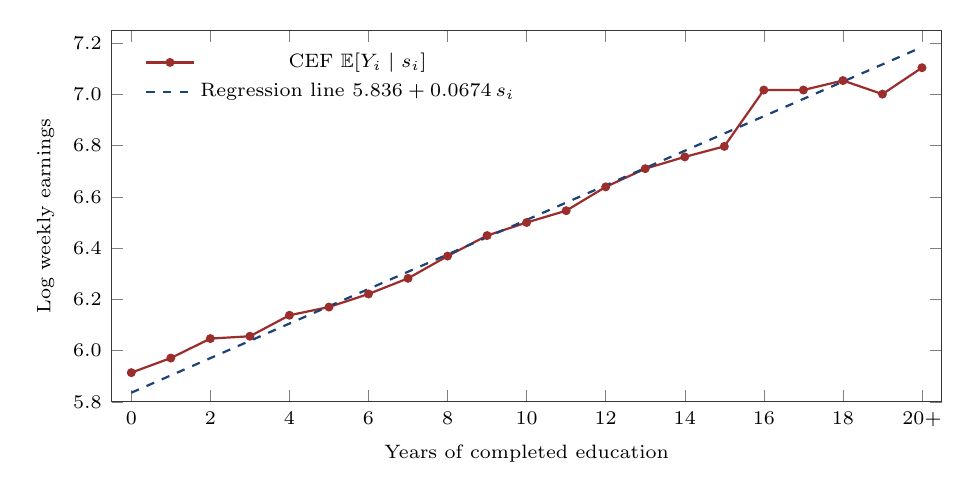
\begin{tikzpicture}
\begin{axis}[
    width=\linewidth, height=6.3cm,
    xmin=-0.5, xmax=20.5, ymin=5.8, ymax=7.25,
    xtick={0,2,...,20},
    xticklabels={0,2,4,6,8,10,12,14,16,18,20+},
    ytick={5.8,6.0,6.2,6.4,6.6,6.8,7.0,7.2},
    yticklabel style={/pgf/number format/.cd,fixed,fixed zerofill,precision=1},
    tick label style={font=\scriptsize},
    label style={font=\scriptsize},
    xlabel={Years of completed education},
    ylabel={Log weekly earnings},
    legend pos=north west,
    legend style={font=\scriptsize, draw=none, fill=none},
    axis line style={DarkGray},
]
  \addplot[DarkRed, thick, mark=*, mark size=1.2pt] coordinates {
      (0,5.914) (1,5.971) (2,6.047) (3,6.056) (4,6.138) (5,6.170)
      (6,6.221) (7,6.282) (8,6.369) (9,6.449) (10,6.500) (11,6.546)
      (12,6.639) (13,6.710) (14,6.756) (15,6.797) (16,7.017) (17,7.017)
      (18,7.054) (19,7.001) (20,7.104)};
  \addlegendentry{CEF $\E[Y_i\mid s_i]$}
  \addplot[DeepBlue, thick, dashed, domain=0:20, samples=2]
      {5.835761+0.0674387*x};
  \addlegendentry{Regression line $5.836+0.0674\,s_i$}
\end{axis}
\end{tikzpicture}

\vspace{-0.3em}
\Src{CEF values approximated from MHE Fig.\ 3.1.2; line uses the
coefficients reported in Fig.\ 3.1.3.}
\end{column}

\begin{column}{0.40\textwidth}
\begin{itemize}
    \item Same schooling CEF as in Fig.\ 3.1.1.
    \item The regression line fits the somewhat bumpy, nonlinear CEF
    \alert{as if we were estimating a model for $\E[Y_i\mid X_i]$ instead of
    a model for $Y_i$}.
    \item That is exactly what is going on (Theorem 3.1.6).
\end{itemize}

\medskip

\begin{block}{Implication}
Regression coefficients can be obtained using $\E[Y_i\mid X_i]$ as the
dependent variable instead of $Y_i$ itself.
\end{block}
\end{column}
\end{columns}

\end{frame}


% ------------------------------------------------------------
\begin{frame}{Regressing the CEF: Grouped Data}
\small

Suppose $X_i$ is discrete with probability mass function $g_x(u)$. Then
\[
\E\big\{(\E[Y_i\mid X_i]-X_i'b)^2\big\}
= \sum_u \big(\E[Y_i\mid X_i=u]-u'b\big)^2\, g_x(u).
\]
$\Rightarrow$ $\beta$ is the \textbf{weighted least squares} regression of
$\E[Y_i\mid X_i=u]$ on $u$, where $u$ runs over the values of $X_i$ and the
weights are the distribution of $X_i$, $g_x(u)$.

\medskip

An even simpler way to see it --- iterate expectations in the formula for
$\beta$:
\[
\boxed{
\beta = \E[X_iX_i']^{-1}\E[X_iY_i]
      = \E[X_iX_i']^{-1}\E\big[X_i\,\E(Y_i\mid X_i)\big]
}
\tag{3.1.5}
\]

\begin{block}{Practical use: when microdata are unavailable}
Angrist (1998) studies the effect of voluntary military service on later
civilian earnings, regressing earnings on a veteran dummy, personal
characteristics, and the variables the military uses to screen soldiers.
Social Security earnings records cannot be released, so the analysis uses
\alert{average earnings} conditional on race, sex, test scores, education,
and veteran status.
\end{block}

\end{frame}


% ------------------------------------------------------------
\begin{frame}{Microdata vs.\ Grouped Data (Fig.\ 3.1.3)}
\small

Returns to schooling, white men aged 40--49, 1980 Census (IPUMS 5\%);
robust SEs are heteroskedasticity consistent.

\begin{center}
\footnotesize
\renewcommand{\arraystretch}{1.1}
\begin{tabular}{@{}lccccccc@{}}
\toprule
 & Coef. & Robust SE & Conv.\ SE & Robust $t$ & $N$ & $R^2$ & Root MSE \\
\midrule
\multicolumn{8}{@{}l}{\textbf{A. Individual-level data}} \\
\quad school & .0674387 & .0003447 & .0003043 & 195.63 & 409{,}435 & .1071 & .67879 \\
\quad const. & 5.835761 & .0045507 & .0040043 & 1282.39 & & & \\
\midrule
\multicolumn{8}{@{}l}{\textbf{B. Means by years of schooling}} \\
\quad school & .0674387 & .0040352 & .0029013 & 16.71 & 21 & .9660 & .04635 \\
\quad const. & 5.835761 & .0399452 & .0381792 & 146.09 & & & \\
\bottomrule
\end{tabular}

\vspace{0.2em}
\Src{Stata: (A) \texttt{regress earnings school, robust};\quad
(B) \texttt{regress average\_earnings school [aweight=count], robust}.}
\end{center}

\begin{itemize}
    \item \textbf{Coefficients are identical}: 21 conditional means,
    weighted by the number of individuals at each schooling level, reproduce
    the estimates from hundreds of thousands of observations.
    \item \textbf{Standard errors are not}: grouped-regression SEs do not
    measure the asymptotic sampling variance of the slope in repeated
    micro-data samples. That requires the variance of $Y_i-X_i'\beta$, which
    depends on the microdata --- the second moments of
    $W_i\equiv[Y_i\ X_i']'$ ($\rightarrow$ next section).
\end{itemize}

\end{frame}


% ============================================================
% SECTION 4: ASYMPTOTIC OLS INFERENCE
% ============================================================

\section{Asymptotic OLS Inference}

% ------------------------------------------------------------
\begin{frame}{From Population to Sample: OLS as a Method of Moments}
\small

In practice we know neither the CEF nor $\beta$, so we draw inferences from
samples. Key point: \alert{inference is distinct from interpretation}.
Whatever a regression coefficient may mean, it has a sampling distribution
that is easy to describe and use. \Src{(Condensed from Chamberlain 1984.)}

\medskip

\textbf{Setup.} $W_i\equiv[Y_i\ X_i']'$ is i.i.d.\ in a sample of size $N$.
\begin{itemize}
    \item Sample moments estimate population moments:
    $\frac1N\sum_i W_i$ for $\E[W_i]$, $\frac1N\sum_i W_iW_i'$ for
    $\E[W_iW_i']$, and so on (law of large numbers).
    \item \textbf{Method of moments:} replace each expectation in
    $\beta=\E[X_iX_i']^{-1}\E[X_iY_i]$ by a sum:
    \[
    \boxed{
    \hat\beta = \Big[\sum_i X_iX_i'\Big]^{-1}\sum_i X_iY_i
    }
    \]
    \item Called \textbf{OLS} because it also solves the sample analog of
    the least squares problem (3.1.2).
    \item Matrix form: with $X$ the matrix with rows $X_i'$ and $y$ the vector
    of $Y_i$, $\frac1N\sum_iX_iX_i'=X'X/N$ and $\frac1N\sum_iX_iY_i=X'y/N$, so
    $\hat\beta=(X'X)^{-1}X'y$.
\end{itemize}

\medskip

The asymptotic distribution of $\hat\beta$ depends only on the definition of
the estimand ($\beta$) and the assumption of random sampling.

\end{frame}


% ------------------------------------------------------------
\begin{frame}{The Asymptotic Toolkit}
\small

{\footnotesize
\renewcommand{\arraystretch}{1.15}
\noindent
\begin{tabular}{@{}B{1.8cm}L{6.3cm}L{6.1cm}@{}}
\toprule
Result & In words & Formally \\
\midrule
LLN
  & Sample moments converge in probability to the corresponding population
    moments.
  & $\frac1N\sum_iW_i\pto\E[W_i]$ \\
CLT
  & Centered, $\sqrt N$-scaled sample moments are asymptotically normal,
    with the covariance of the underlying variable.
  & $\sqrt N\big(\frac1N\sum_iW_i-\E[W_i]\big)\dto N\big(0,\Var(W_i)\big)$ \\
Slutsky
  & If $a_N$ has an asymptotic distribution and $b_N\pto b$, then $b_N$ can
    be replaced by $b$ in sums and products.
  & $a_N+b_N$ and $a_N+b$ (likewise $a_Nb_N$ and $a_Nb$) have the same
    asymptotic distribution \\
Continuous mapping
  & Probability limits pass through continuous functions.
  & $\plim h(b_N)=h(b)$ if $\plim b_N=b$ and $h$ is continuous at $b$ \\
Delta method
  & Continuously differentiable functions of asymptotically normal
    variables are asymptotically normal (covariance: a quadratic form, with
    the gradient outside).
  & $\sqrt N\big(h(b_N)-h(b)\big)\dto N\big(0,\nabla h(b)'\Omega\nabla h(b)\big)$,
    where $\Omega$ is the asymptotic covariance matrix of $b_N$ \\
\bottomrule
\end{tabular}
\par}

\smallskip

\Src{Quadratic form: for diagonal $M$, $v'Mv=\sum_i m_iv_i^2$.\quad
\emph{Consistent} $=$ converges in probability to the target.\quad
Formal statements: Knight (2000).}

\end{frame}


% ------------------------------------------------------------
\begin{frame}{The Asymptotic Distribution of $\hat\beta$ (I): Setup}
\small

\textbf{Two routes:}
\begin{itemize}
    \item \textbf{Delta method:} $\hat\beta$ is a function of sample moments,
    hence asymptotically normal; it remains to find the covariance matrix from
    the gradient of this function (consistency follows from the CMT).
    Conceptually straightforward but somewhat inelegant.
    \item \textbf{Slutsky $+$ CLT:} easier and more instructive
    $\Rightarrow$ the route taken here.
\end{itemize}

\medskip

\textbf{Step 1.} Write
\[
Y_i = X_i'\beta+[Y_i-X_i'\beta]\equiv X_i'\beta+e_i.
\tag{3.1.6}
\]

\begin{alertblock}{$\E[X_ie_i]=0$ is a consequence, not an assumption}
It follows from $\beta=\E[X_iX_i']^{-1}\E[X_iY_i]$ and $e_i=Y_i-X_i'\beta$,
not from an assumption about an underlying economic relation. Residuals
defined this way need not be mean independent of $X_i$ --- for that we need a
linear CEF.
\end{alertblock}

\medskip

\textbf{Step 2.} Substitute (3.1.6) for $Y_i$ in the formula for $\hat\beta$:
\[
\hat\beta = \beta+\Big[\sum_iX_iX_i'\Big]^{-1}\sum_iX_ie_i.
\]

\end{frame}


% ------------------------------------------------------------
\begin{frame}{The Asymptotic Distribution of $\hat\beta$ (II): Slutsky and the CLT}
\small

\textbf{Step 3.} The asymptotic distribution of $\hat\beta$ is that of
\[
\sqrt N(\hat\beta-\beta)
= N\Big[\sum_iX_iX_i'\Big]^{-1}\frac{1}{\sqrt N}\sum_iX_ie_i
= \Big[\frac1N\sum_iX_iX_i'\Big]^{-1}\frac{1}{\sqrt N}\sum_iX_ie_i.
\]
\begin{itemize}
    \item \textbf{Slutsky:} $\frac1N\sum_iX_iX_i'\pto\E[X_iX_i']$, so this has
    the same asymptotic distribution as
    $\E[X_iX_i']^{-1}\frac{1}{\sqrt N}\sum_iX_ie_i$.
    \item \textbf{CLT:} since $\E[X_ie_i]=0$,
    $\frac{1}{\sqrt N}\sum_iX_ie_i$ is a root-$N$ normalized, centered sample
    moment, so
    $\frac{1}{\sqrt N}\sum_iX_ie_i\dto N\big(0,\E[X_iX_i'e_i^2]\big)$ ---
    the covariance matrix of $X_ie_i$, a matrix of fourth moments.
\end{itemize}

\medskip

\begin{block}{Result}
$\hat\beta$ is asymptotically normal with probability limit $\beta$ and
asymptotic covariance matrix
\[
\E[X_iX_i']^{-1}\,\E[X_iX_i'e_i^2]\,\E[X_iX_i']^{-1}.
\tag{3.1.7}
\]
\end{block}

\end{frame}


% ------------------------------------------------------------
\begin{frame}{Robust Standard Errors}
\small

\begin{itemize}
    \item Theoretical standard errors for $t$-statistics are the square roots
    of the diagonal elements of (3.1.7) (divided by $N$).
    \item In practice: replace expectations by sums and $e_i$ by the
    estimated residuals $\hat e_i=Y_i-X_i'\hat\beta$, giving the empirical
    fourth-moment matrix $\sum_i[X_iX_i'\hat e_i^2]/N$:
    \[
    \widehat{\Var}(\hat\beta)
    = \Big[\sum_iX_iX_i'\Big]^{-1}
      \Big[\sum_iX_iX_i'\hat e_i^2\Big]
      \Big[\sum_iX_iX_i'\Big]^{-1}.
    \]
\end{itemize}

\begin{block}{Many names, one object}
Heteroskedasticity-consistent standard errors; White (1980a) standard errors;
Eicker--White standard errors (Eicker 1967); ``robust'' standard errors
(e.g., in Stata).
\end{block}

\medskip

\textbf{Why ``robust''?} In large samples they deliver accurate hypothesis
tests and confidence intervals under minimal assumptions about the data and
model: the derivation assumed nothing beyond what is needed for basic results
like the CLT to go through.

\begin{alertblock}{But\ldots}
Robust standard errors are \emph{not} the default in packaged software.
\end{alertblock}

\end{frame}


% ------------------------------------------------------------
\begin{frame}{Conventional Standard Errors and Why Heteroskedasticity Is Natural}
\small

\textbf{Default SEs assume homoskedasticity:} $\E[e_i^2\mid X_i]=\sigma^2$,
a constant. Iterating expectations,
$\E[X_iX_i'e_i^2]=\E\big(X_iX_i'\E[e_i^2\mid X_i]\big)=\sigma^2\E[X_iX_i']$,
so (3.1.7) simplifies to
\[
\E[X_iX_i']^{-1}\sigma^2\E[X_iX_i']\E[X_iX_i']^{-1}
= \sigma^2\E[X_iX_i']^{-1}.
\tag{3.1.8}
\]
Its diagonal elements are what SAS and Stata report unless asked otherwise.

\smallskip

\textbf{But viewing regression as an approximation to the CEF makes
heteroskedasticity natural.}
\begin{itemize}
    \item If the CEF is nonlinear, the quality of the linear fit varies with
    $X_i$: residuals are larger, on average, where the fit is poorer.
    \item Even if $\Var(Y_i\mid X_i)$ is constant:
    \[
    \begin{aligned}
    \E[(Y_i-X_i'\beta)^2\mid X_i]
    &= \E\big\{[(Y_i-\E[Y_i\mid X_i])+(\E[Y_i\mid X_i]-X_i'\beta)]^2\,\big|\,X_i\big\}\\
    &= \Var(Y_i\mid X_i)+(\E[Y_i\mid X_i]-X_i'\beta)^2,
    \end{aligned}
    \tag{3.1.9}
    \]
    where the cross term vanishes because $Y_i-\E[Y_i\mid X_i]$ is mean
    independent of $X_i$.
\end{itemize}

\begin{block}{}
Residual variance rises with the \alert{squared gap between the regression
line and the CEF} \Src{(White 1980b)}.
\end{block}

\end{frame}


% ------------------------------------------------------------
\begin{frame}{Heteroskedasticity: The LPM, and Does It Matter?}
\small

\textbf{A linear CEF makes homoskedasticity possible, but is not
sufficient.} Example: the \emph{linear probability model} (LPM), i.e.\ any
regression with a 0--1 dependent variable (e.g., labor force
participation).
\begin{itemize}
    \item With a saturated model the CEF is linear, so the residual variance
    equals the conditional variance $\Var(Y_i\mid X_i)$.
    \item But $Y_i$ is Bernoulli:
    $\Var(Y_i\mid X_i)=P[Y_i=1\mid X_i]\,(1-P[Y_i=1\mid X_i])$
    $\Rightarrow$ LPM residuals are necessarily heteroskedastic unless the
    only regressor is a constant.
\end{itemize}

\medskip

\textbf{In practice, heteroskedasticity may matter little} (schooling
coefficient, Fig.\ 3.1.3):
\begin{itemize}
    \item Microdata: robust SE $.0003447$ vs.\ conventional $.0003043$ ---
    not much smaller.
    \item Grouped data (necessarily heteroskedastic if group sizes differ):
    robust $.004$ vs.\ conventional $.0029$ --- somewhat more different.
\end{itemize}

\begin{alertblock}{Rules of thumb (such differences are typical)}
\begin{itemize}
    \item If robust SEs are, say, $>30\%$ larger than conventional ones, or
    markedly smaller, worry about programming errors or other problems.
    \item Robust SEs below conventional ones may signal finite-sample bias in
    the robust calculation.
\end{itemize}
\end{alertblock}

\end{frame}


% ------------------------------------------------------------
\begin{frame}{Asymptotic vs.\ the Textbook (Classical) Approach}
\small

Traditional econometric inference begins with \emph{stronger} assumptions
than those invoked so far \Src{(see, e.g., Goldberger 1991)}.

\medskip

\begin{columns}[T]
\begin{column}{0.49\textwidth}
\begin{block}{Classical normal regression model}
Assumes
\begin{itemize}
    \item fixed (non-stochastic) regressors,
    \item a linear CEF,
    \item normally distributed errors,
    \item homoskedasticity.
\end{itemize}
Delivers
\begin{enumerate}
    \item unbiasedness, $\E[\hat\beta]=\beta$, in a sample of any size ---
    stronger than consistency;
    \item a sampling-variance formula valid in small and large samples.
\end{enumerate}
\end{block}
\end{column}
\begin{column}{0.49\textwidth}
\begin{block}{When is OLS unbiased?}
\[
\E[\hat\beta]
= \beta+\E\Big\{\Big[\sum_iX_iX_i'\Big]^{-1}\sum_iX_ie_i\Big\}.
\]
\begin{itemize}
    \item Non-random regressors: the expectation passes through and
    $\E[e_i]=0$.
    \item Random regressors: iterate expectations; unbiased if
    $\E[e_i\mid X_i]=0$ --- true when the CEF is linear, but \alert{not} in
    the general ``agnostic regression'' framework.
\end{itemize}
\end{block}
\end{column}
\end{columns}

\end{frame}


% ------------------------------------------------------------
\begin{frame}{Why Start from Asymptotics?}
\small

\begin{block}{Same variance formula, different claims}
The variance formula obtained under the classical assumptions is the same as
the large-sample formula under homoskedasticity, (3.1.8) --- but, provided
the strong classical assumptions are valid, it holds in a sample of
\emph{any} size.
\end{block}

\medskip

\begin{block}{Why the asymptotic approach here}
\begin{itemize}
    \item Modern empirical work leans heavily on the large-sample theory
    behind robust variance formulas.
    \item Payoff: valid inference under weak assumptions --- in particular,
    a framework that makes sense for a less-than-literal approach to
    regression models (regression as an approximation to the CEF).
\end{itemize}
\end{block}

\medskip

\begin{alertblock}{Caveat}
The large-sample approach is not without its dangers $\rightarrow$
inference in Chapter~8 and instrumental variables in Chapter~4.
\end{alertblock}

\end{frame}


% ============================================================
% SUMMARY
% ============================================================

\section{Summary}

\begin{frame}{Summary: Regression Fundamentals}
\small

\begin{enumerate}
    \item \textbf{The CEF} $\E[Y_i\mid X_i]$ summarizes ``systematic
    randomness.'' By the LIE it yields
    $Y_i=\E[Y_i\mid X_i]+\varepsilon_i$ with $\varepsilon_i$ orthogonal to any
    $h(X_i)$; it is the MMSE predictor; and
    $\Var(Y_i)=\Var(\E[Y_i\mid X_i])+\E[\Var(Y_i\mid X_i)]$. None of this
    needs linearity.
    \item \textbf{Population regression}
    $\beta=\E[X_iX_i']^{-1}\E[X_iY_i]$ is a nonstochastic feature of the
    population; $\E[X_ie_i]=0$ holds by construction. Anatomy:
    $\beta_k=\Cov(Y_i,\tilde x_{ki})/\Var(\tilde x_{ki})$.
    \item \textbf{Why regression?} (I) If the CEF is linear --- e.g., in a
    saturated model --- regression \emph{is} the CEF; (II) $X_i'\beta$ is the
    best linear predictor of $Y_i$; (III) $X_i'\beta$ is the best linear
    approximation to the CEF, so $\beta$ can be computed from the CEF itself
    (grouped data / WLS).
    \item \textbf{Saturated models} fit the CEF exactly via main effects and
    interactions; restricted (e.g., additive) models approximate it.
    \item \textbf{Inference:} $\hat\beta$ is the method-of-moments analog of
    $\beta$; it is asymptotically normal with sandwich covariance
    $\E[X_iX_i']^{-1}\E[X_iX_i'e_i^2]\E[X_iX_i']^{-1}$. Robust SEs need
    minimal assumptions, and heteroskedasticity is the natural case.
\end{enumerate}

\medskip

\[
\boxed{
\text{Regression is always a good summary of the CEF.
\emph{When} is it causal? \;$\rightarrow$\; \Sec{}3.2}
}
\]

\end{frame}


% ------------------------------------------------------------
\begin{frame}{References Cited in \Sec{}3.1}
\scriptsize

\begin{itemize}
    \item Angrist, J. D. (1998). ``Estimating the Labor Market Impact of
    Voluntary Military Service Using Social Security Data on Military
    Applicants.'' \emph{Econometrica}, 66(2), 249--288.
    \item Autor, D. H., L. F. Katz, and M. S. Kearney (2005). ``Rising Wage
    Inequality: The Role of Composition and Prices.'' NBER Working Paper
    11628.
    \item Chamberlain, G. (1984). ``Panel Data.'' In Z. Griliches and
    M. D. Intriligator (eds.), \emph{Handbook of Econometrics}, Vol.~2.
    \item Eicker, F. (1967). ``Limit Theorems for Regressions with Unequal and
    Dependent Errors.'' \emph{Proceedings of the Fifth Berkeley Symposium on
    Mathematical Statistics and Probability}, Vol.~1, 59--82.
    \item Frisch, R., and F. V. Waugh (1933). ``Partial Time Regressions as
    Compared with Individual Trends.'' \emph{Econometrica}, 1(4), 387--401.
    \item Galton, F. (1886). ``Regression Towards Mediocrity in Hereditary
    Stature.'' \emph{Journal of the Anthropological Institute of Great
    Britain and Ireland}, 15, 246--263.
    \item Goldberger, A. S. (1991). \emph{A Course in Econometrics}. Harvard
    University Press.
    \item Knight, K. (2000). \emph{Mathematical Statistics}. Chapman \&
    Hall/CRC.
    \item Manski, C. F. (1991). ``Regression.'' \emph{Journal of Economic
    Literature}, 29(1), 34--50.
    \item White, H. (1980a). ``A Heteroskedasticity-Consistent Covariance
    Matrix Estimator and a Direct Test for Heteroskedasticity.''
    \emph{Econometrica}, 48(4), 817--838.
    \item White, H. (1980b). ``Using Least Squares to Approximate Unknown
    Regression Functions.'' \emph{International Economic Review}, 21(1),
    149--170.
\end{itemize}

\end{frame}

\end{document}
